\section{Evaluation of Environmental Wireless Sensor Networks (E-WSN)}
\label{section:experimental}	
\begin{figure}[ht]
	\centering
	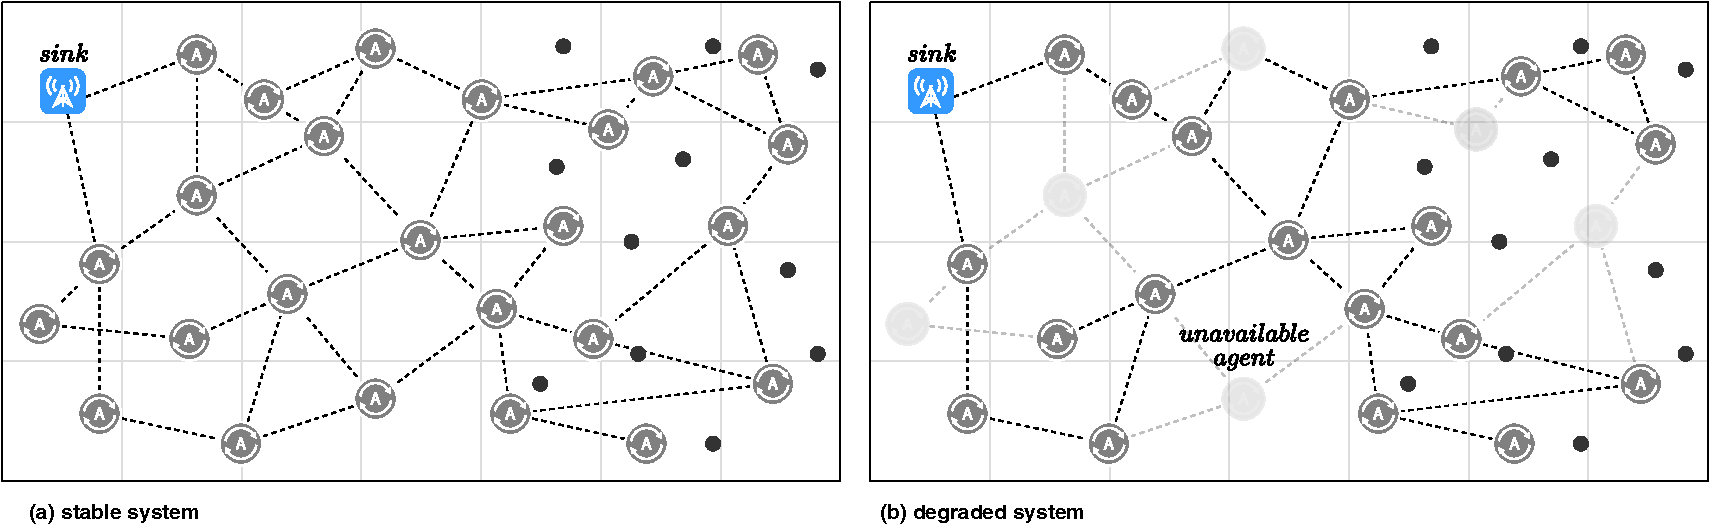
\includegraphics[width=0.9\linewidth, trim={25pt 0pt 25pt 0pt, clip}]{system-types}
	\caption{\textbf{System types}. The diagram shows examples of two systems. In the first \simulationSimple{}{}, there are $10$ possible agents that can execute the measurement task, tasks' demand points are distributed across the map. In the second, \simulationExtended{}{} system, there are $25$ agents that can execute the measurement tasks. The tasks' demand points are clustered away from the sink node.}
	\label{fig:system-types}
\end{figure}
\begin{figure}[ht]
	\centering
	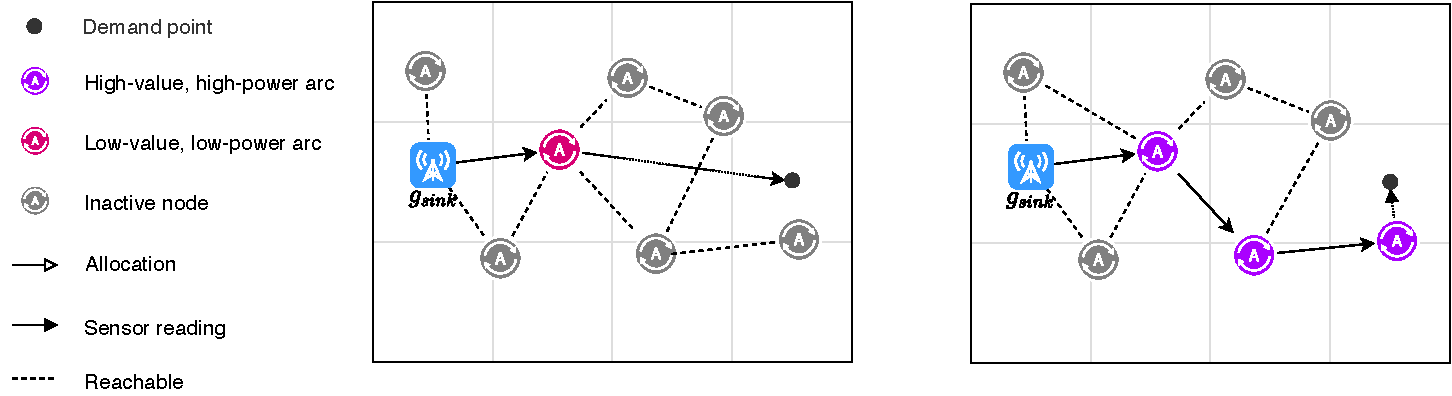
\includegraphics[width=0.9\linewidth, trim={25pt 0pt 25pt 0pt, clip}]{route-types}
	\caption{\textbf{Routes, power consumption, and task value}. The diagram shows two possible task-paths for the same system. In the first, energy is conserved by having a short task-path but the task is completed to a lesser quality. In the second, the maximum quality for the task is achieved, however, there is more energy consumption overall.}
	\label{fig:route_types}
\end{figure}

The simulation framework to evaluate the algorithms' performance was based on a realistic deployment scenario as covered by  \cite{Gomez2015} and others \citep{Jha2016, Avram}. In this scenario a UAV is used to deploy a large number of sensors over a expansive and remote geographical area, giving an ad-hoc, randomised placement of devices. Solar power cells are used to maintain enough energy to power the sensors over a number of years, given low enough power consumption. 

We simulated three systems and evaluated the algorithm in different configurations (See Figure \ref{fig:system-types}).  
\begin{enumerate}
	\item The \simulationSimple{}{} system simulates a basic environment examining energy and quality optimisation, with  equal weighting for each of the CTV components $\alpha, \beta, \gamma$ (Eq. \ref{eq:ctv}). $1$ sink node and $10$ other nodes were distributed randomly in the system, each one initially connected to $3$ other nodes that were randomly chosen with a bias towards closer located nodes\footnote{
		The probability of initial node selection used the standard gamma distribution $f(x; \alpha, \beta) = \frac{\beta^{\alpha} x^{\alpha-1}e^{- \beta x}}   {\Gamma(\alpha)}$, where $\Gamma(\alpha)$ is the  gamma function, $\alpha=1.8, \beta=0.5$, and $x$ is the unit distance between the two nodes.
	}. 
	The sink node was given $3$ composite tasks to complete sequentially, each consisting of $5$ different atomic measurement tasks. The completion of the $3$ composite tasks marked the end of an episode, and the process was repeated for $1000$ episodes. Each other node was capable of completing an atomic task, or allocating it to any of $3$ nodes it was connected to. They could complete any measurement task with a quality dependent on their closeness to the demand point associated with the task (Eq. \ref{eq:atomic_task_quality}). The energy of all nodes in the system was fully reset at the end of each episode. An example of the simple system layout can be seen in Figure \ref{fig:system-types}(a). 

	\item The \simulationNodeFailure{}{} system introduces degradation of the system over time, showing how each algorithm maintains coverage and optimises for quality and energy while some node availability is lost. It used the configuration of the \simulationSimple{}{} system and added in random node failures. The simulation ran for $100$ episodes, where for each episode between $20$ and $40$  a randomly chosen single node might fail with probability $0.25$. Once a node failed, it was unresponsive for all further episodes. 
	
	\item The \simulationExtended{}{} system is structured to test the algorithms' performance in task-path selection given different configurations. 
	It had CTV component weightings where each of the relevant properties were given an $80\%$ dominance over the value of CTV value. $1$ sink node was given a composite task consisting of $10$ atomic task measurements to complete. It was placed at a significantly large distance from the demand points associated with the atomic tasks. $25$ nodes were distributed randomly in the system. This system examined the impact of the algorithm optimising the allocation of tasks towards the goals stated in Section \ref{section:optimisation_problem}. Atomic task quality could be maximised, but at the cost of longer task-paths and therefore energy usage, or energy consumption could be minimised, with correspondingly lower task qualities. Figure \ref{fig:route_types} illustrates these two route types for task completion.
\end{enumerate}
  As a comparison we use the \acronymQRouting{}{} algorithm, a Q-learning based algorithm  used to optimise network routes based on energy consumption and task quality equally \citep{XXX, XXX}.